 \chapter{Desenvolvimento}
\label{cap:desenv}

% - - - - - - - - - - - - - - - - - - - - - - - - - - - - - - - - - - -
\section{Abordagem Inicial}
\label{sec:abord-ini} 
Neste capítulo será abordado todos os passos realizados para se alcançar o objetivo esperado deste trabalho. Para desenvolvimento foi utilizado a linguagem de programação Python por  ter sintaxe simples e suporte a biblioteca OPenCV (\textit{Open Source Computer Vision}) a qual possui diversas técnicas eficientes  e robustas voltadas para processamento de imagens, visão computacional e com  foco em aplicações em tempo real.

Neste trabalho foi utilizado para captura das imagens um iphone 5 resolução da câmera ( 3264 x 2448 pixel) e posteriormente um 6s (4608 x 2592 pixel). A ideia é que, futuramente esse protótipo possa funcionar em qualquer smartphone sem a necessidade de compra de um hardware especial como acontece em \cite{skip2018} que utiliza scanners específicos para ler os palos.

A abordagem deste trabalho é direcionada na utilização de algoritmos de processamento de imagens e visão computacional para ler uma imagem de um teste palográfico e realizar a contagem dos palos, disponibilizando uma análise quantitativa em tempo real, otimizando o trabalho de correção dos testes.

\section{Visão geral do protótipo}
\label{sec:visao-geral}

Os passos de execução  do algoritmo segue a seguinte ordem:
Carregar a Imagem, Localização da folha, Pré-processamento, Segmentação, Identificação dos palos e Contagem. A Figura \ref{fig:visao-geral} mostra esse processo.

\begin{figure}[H]
 \centering
 \includegraphics[width=0.76\textwidth]{./fig/desenvolvimento/visao-geral}
 \caption{Fluxo do processo para contagem dos palos.}
 \label{fig:visao-geral}
\end{figure}

Na etapa de carregamento a imagem que contém o teste palográfico é carregada na memória e redimensionada, em seguida é repassada para a o pré-processamento e segmentação no qual são aplicados filtros e transformações na imagem para facilitar na etapa de localização  da folha nessa etapa é feito a separação dos objetos  do fundo da imagem e extração do ROI(Região de Interesse) que é a nossa folha do teste palográfico na próxima etapa é aplicado novamente o pré-processamento e segmentação porém dessa vez somente na ROI onde são extraídos os objetos em forma de retângulos que são adicionados em uma lista e repassados para a fase de identificação dos palos onde são feitas validações para identificar os palos. 

No final é feito a contagem dos palos na ordem considerando o intervalo dos 5 tempos. Nas seções seguintes será abordado com mais detalhes os processos descritos.

\section{Carregamento da imagem}
\label{sec:carrega-imagem}
Este trabalho tem o propósito de contar os palos em uma imagem capturada por celular, no entanto, não será desenvolvido nenhum aplicativo para celular apenas o algoritmo de visão computacional para realizar a contagem. Neste protótipo as imagens capturadas pelo celular são transferidas para o computador para serem utilizadas no algoritmo. 


\begin{figure}[H]
 \centering
 \includegraphics[width=0.83\textwidth]{./fig/desenvolvimento/teste-palos}
 \caption{Exemplo de teste palográfico capturado por celular.}
 \label{fig:ex-teste-palo}
\end{figure}


\subsection{Restrições}
\label{subsec:restricoes}
Para o funcionamento correto do protótipo alguns cuidados devem ser tomados na captura das imagens, não utilizar o flash do celular, pois isso gera uma imagem com uma luz mais forte em um só ponto, prejudicando o processamento da imagem. A imagem deve ter uma iluminação homogênea como na Figura \ref{fig:ex-teste-palo}, também deve se tomar cuidado para não fazer sombra sobre a imagem e não amassar e nem dobrar a folha do teste.

\section{Localização da folha}
\label{sec:loc-folha}

Nessa etapa para localizar a região onde se encontra a folha com o teste dos palos na imagem foi utilizado diversas técnicas de processamento de imagens. 

\subsection{Pré-processamento}
\label{sec:pre-proce}

Após o carregamento da imagem é aplicado o filtro Gaussiano para redução de ruídos depois é  feito a conversão para o formata HSV, em seguida é feito uma divisão separando as camadas de Tonalidade(\textit{Hue}), Saturação (\textit{Saturation}) e  Brilho (\textit{Value}) da imagem. Na Figura  \ref{fig:subfiguras} pode ser visto a aplicação dessas técnicas.
\begin{figure}[h]
 \centering
  \subfigure[][Exemplo de conversão da imagem para HSV.]
   {
    
    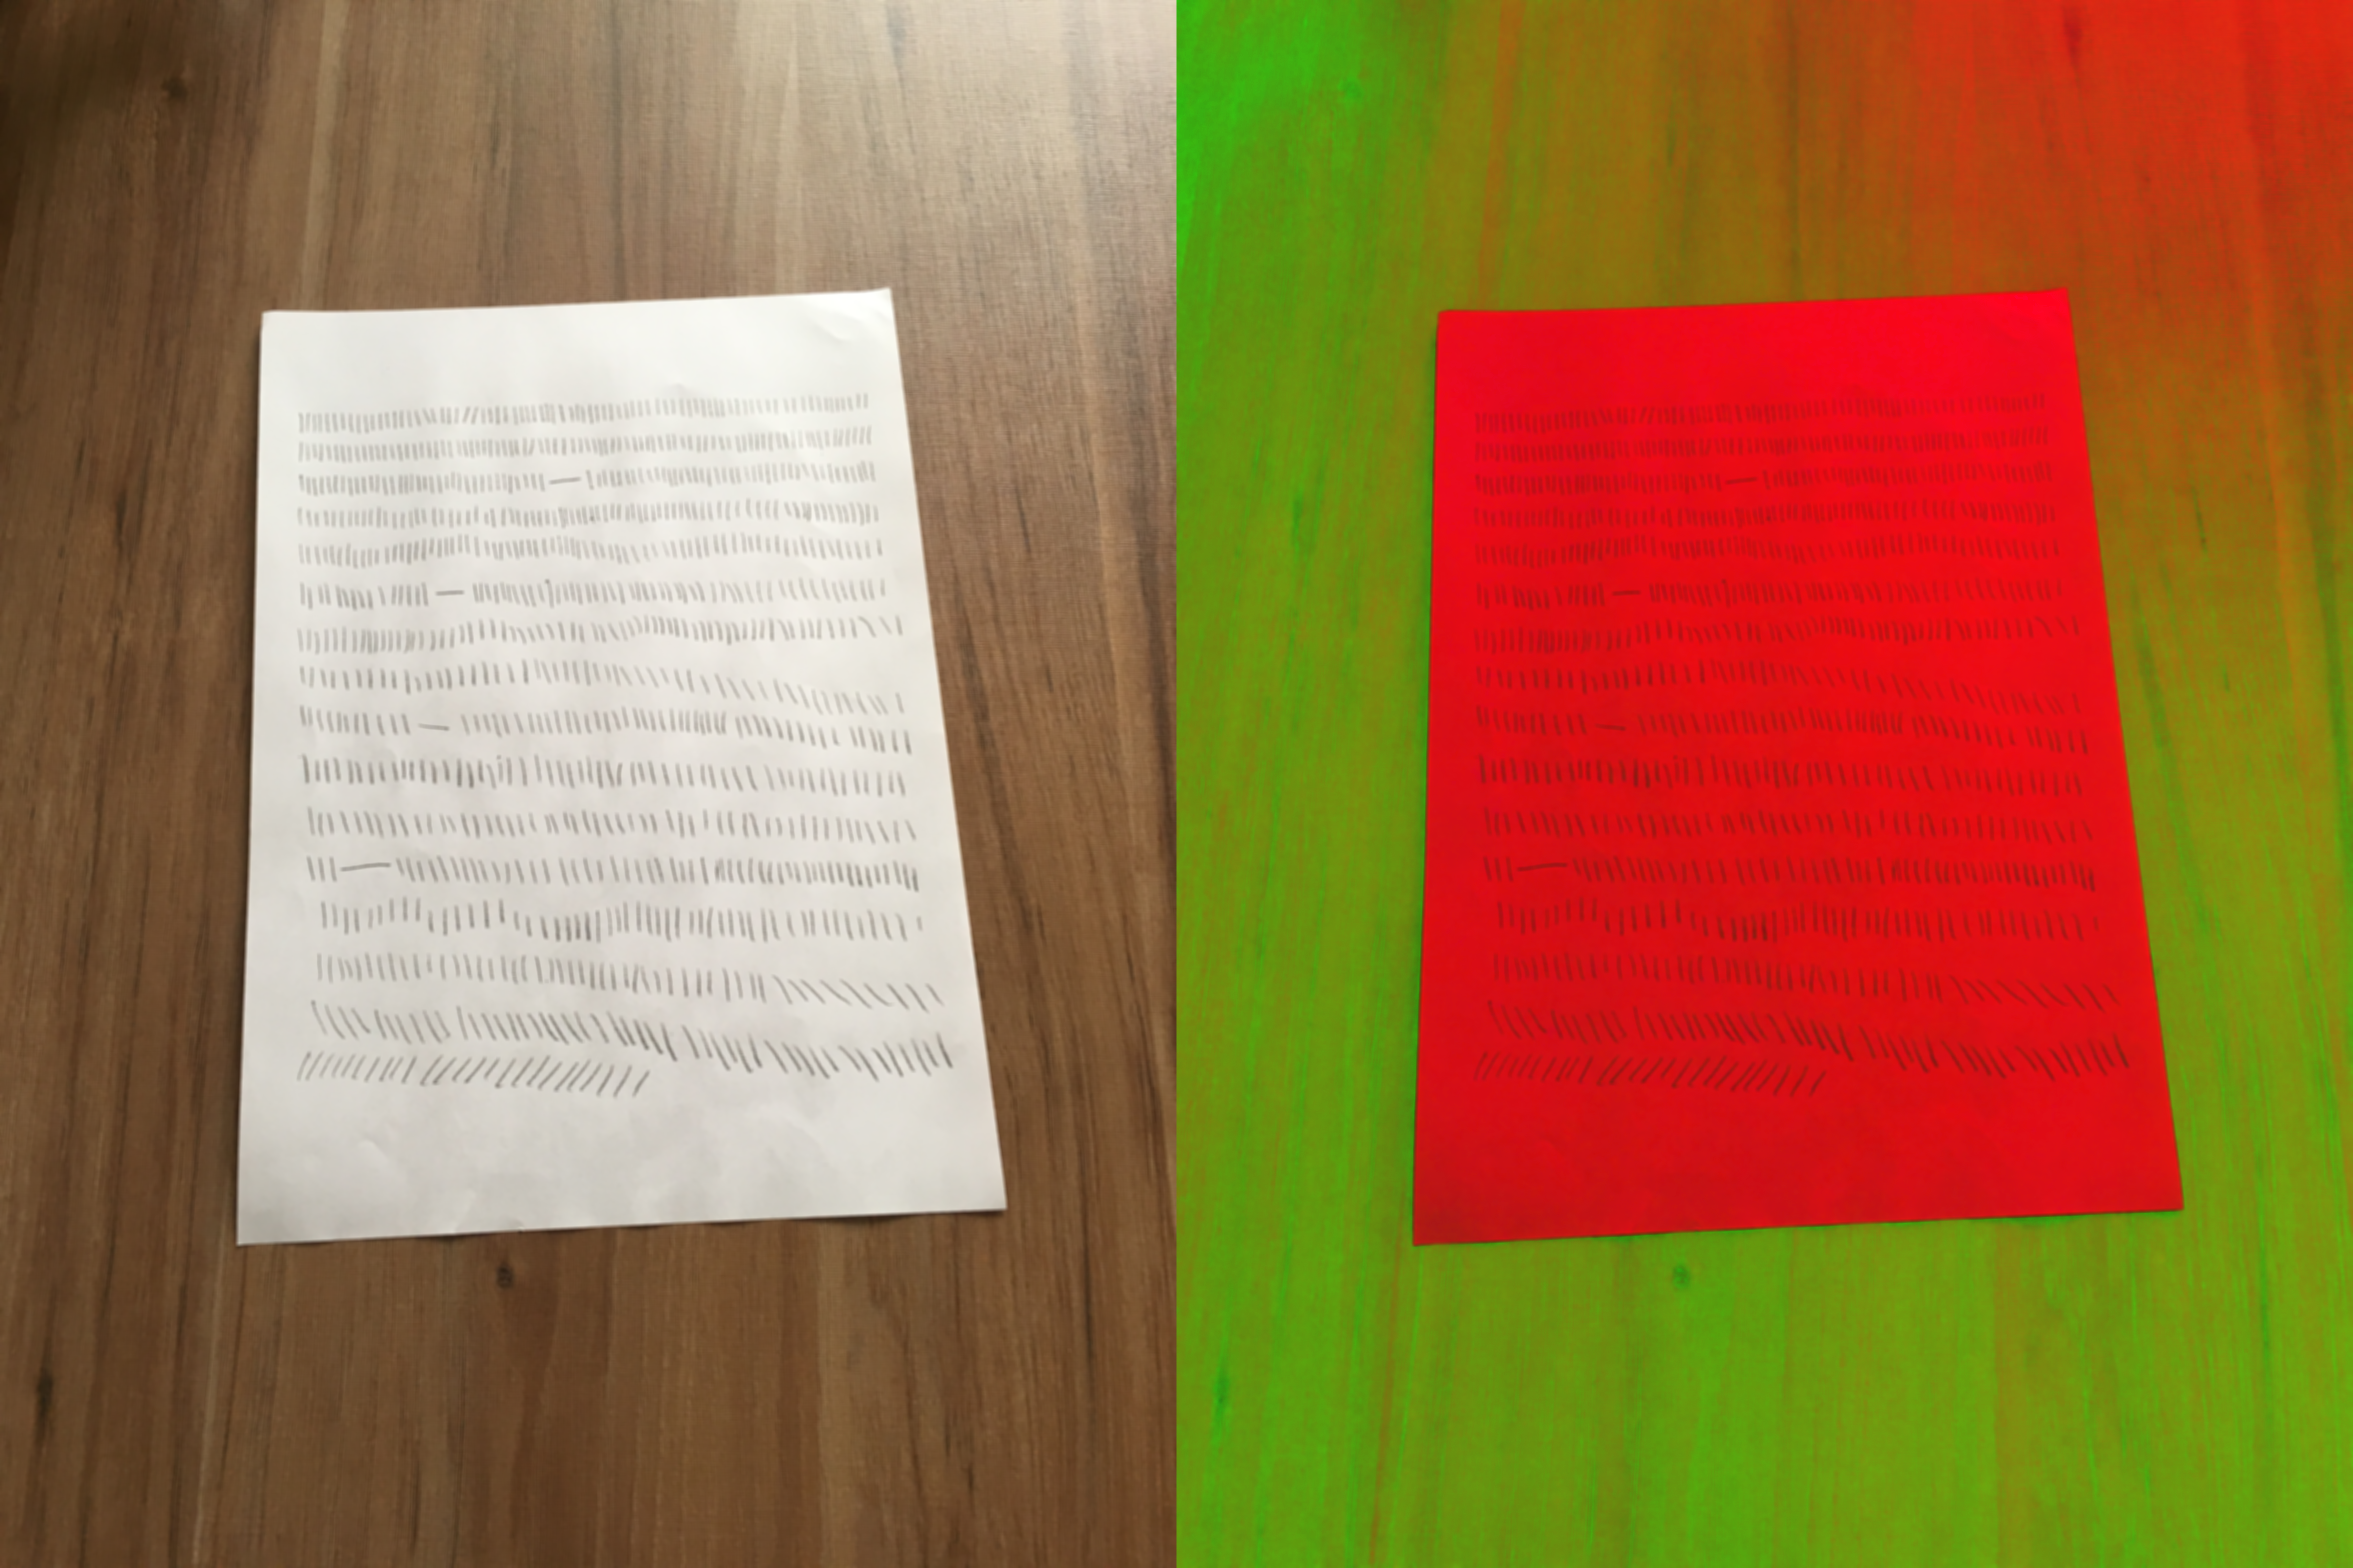
\includegraphics[width=0.25\textwidth]{./fig/desenvolvimento/hsv_x_orig}
    \label{subfig:ex1}
   } \qquad
  \subfigure[Split da imagem separando as camadas Hue, Saturation e Value]
   {
    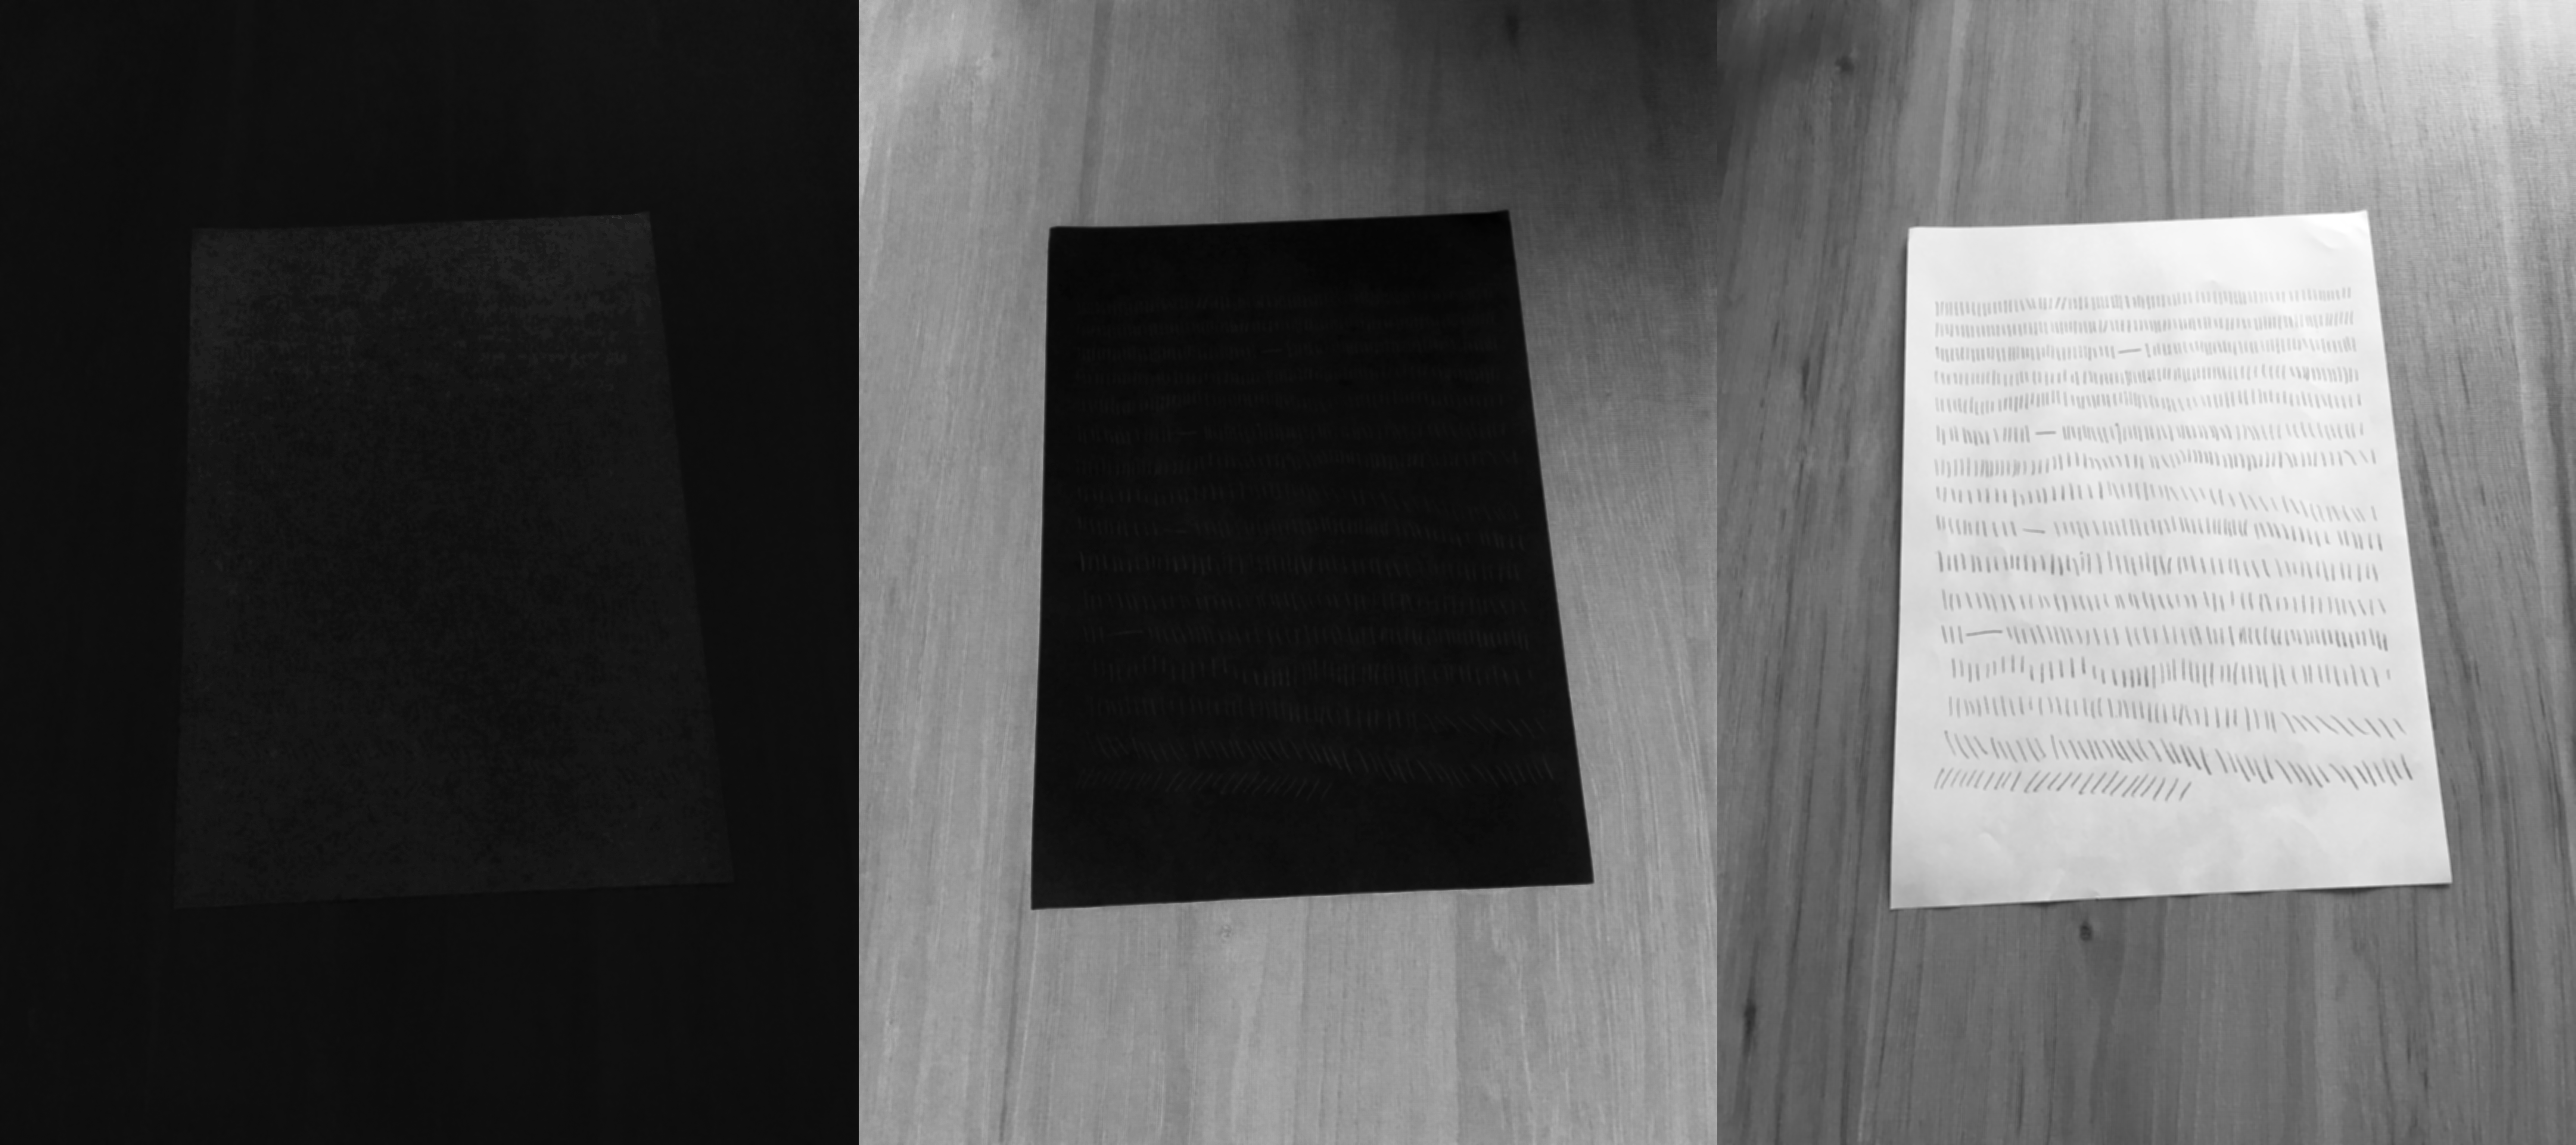
\includegraphics[width=0.37\textwidth]{./fig/desenvolvimento/hsv_split}
    \label{subfig:ex2}
   }
   \caption{{\subref{subfig:ex1}} e {\subref{subfig:ex2}} Resultado do processamento da imagem nessa etapa inicial }
  \label{fig:subfiguras}
\end{figure}
No passo seguinte é aplicado uma transformação morfológica na parte Saturada da imagem,  chamada \textit{Closing} que é uma dilatação seguida de uma erosão. Foi utilizado como teste diversas transformações morfológicas, porém essa foi a que mostrou melhor resultado. Foi realizado uma limiarização (ou binarização) responsável por localizar os objetos presentes na imagem, para isso foram feitos testes com as funções \textbf{threshold} e \textbf{adaptativeThreshold} nativas da biblioteca \textbf{Opencv}, foi obtido  melhor resultado com a função \textbf{adaptativeThreshold}, por trabalhar melhor em imagens com iluminação variável. Os parâmeros utilizados na função foram 255 para o valor máximo, \textbf{ADATIVE THRESH GAUSSIAN C}  para o método, tipo de limiarização \textbf{THRESH BINARY}, 111 para \textbf{Block Size } e 13 para a constante \textbf{C}.
O resultado pode ser visto na Figura  \ref{subfig:adp-thres} 

\begin{figure}[h]
 \centering
  \subfigure[][Imagem binarizada pela função adaptative threshold.]
   {
    
    \includegraphics[width=0.37\textwidth]{./fig/desenvolvimento//adaptative_thres}
    \label{subfig:adp-thres}
   } \qquad
  \subfigure[Detecção de bordas usando o algoritmo Sobel]
   {
    \includegraphics[width=0.37\textwidth]{./fig/desenvolvimento/thresholded_edge_sobel}
    \label{subfig:bordas-sobel}
   }
   \caption{{\subref{subfig:adp-thres}} e {\subref{subfig:bordas-sobel}} Resultado do processamento da imagem }
  \label{fig:subfiguras}
\end{figure}

Podemos notar na Figura \ref{subfig:adp-thres} que o contorno do objeto ficou bem definido agora podemos aplicar os algoritmos para detecção de bordas. Foram testados os algoritmos  Canny e Sobel, sendo o Sobel o que mostrou melhor resultado combinando os filtros horizontal e vertical como pode ser visto na figura \ref{subfig:bordas-sobel}. 

\subsection{Segmentação}
\label{sec:segmentacao}

Após a detecção das bordas com o algoritmo Sobel, foi utilizado a função \textbf{findContours} da Opencv que faz uma varredura na imagem binarizada resultante do processo do Sobel e extrai um vetor de pontos (x,y) do contorno dos objetos encontrados na imagem, os parâmetros que melhor se ajustaram para essa função foram \textbf{RETR EXTERNAL} para o modo de retorno dos contornos e \textbf{CHAIN APPROX SIMPLE} para o método de aproximação dos contornos, isso quer dizer que será retornado os contornos mais externos e com o menor número de pontos possíveis  para identificar a forma presente na imagem isso aumenta a performance do algoritmo. Como na imagem pode haver mais de um objeto ou ruídos, é realizado um cálculo da área de cada objeto e realizado uma ordenação  descendente por área, é feito um laço e validado somente as áreas maiores de 260.000,  em seguida aplico a função  \textbf{approxPolyDP } da Opencv, essa função reduz ainda mais a quantidade de pontos do contorno do objeto, tornando possível identificar o shape do objeto, no nosso caso a folha do teste que tem um formato de retângulo, isso é validado no caso da forma tiver 4 vértices então achamos nosso ROI(Region of interest). Na figura \ref{subfig:roi-img} podemos ver o resultado desse processo, o retângulo verde por cima da folha são as coordenas da ROI.


\begin{figure}[h]
 \centering
  \subfigure[][Localização da região de interesse para segmentação.]
   {
    
    \includegraphics[width=0.37\textwidth]{./fig/desenvolvimento//flat_object_resized_roi}
    \label{subfig:roi-img}
   } \qquad
  \subfigure[Objeto de interesse segmentado.]
   {
    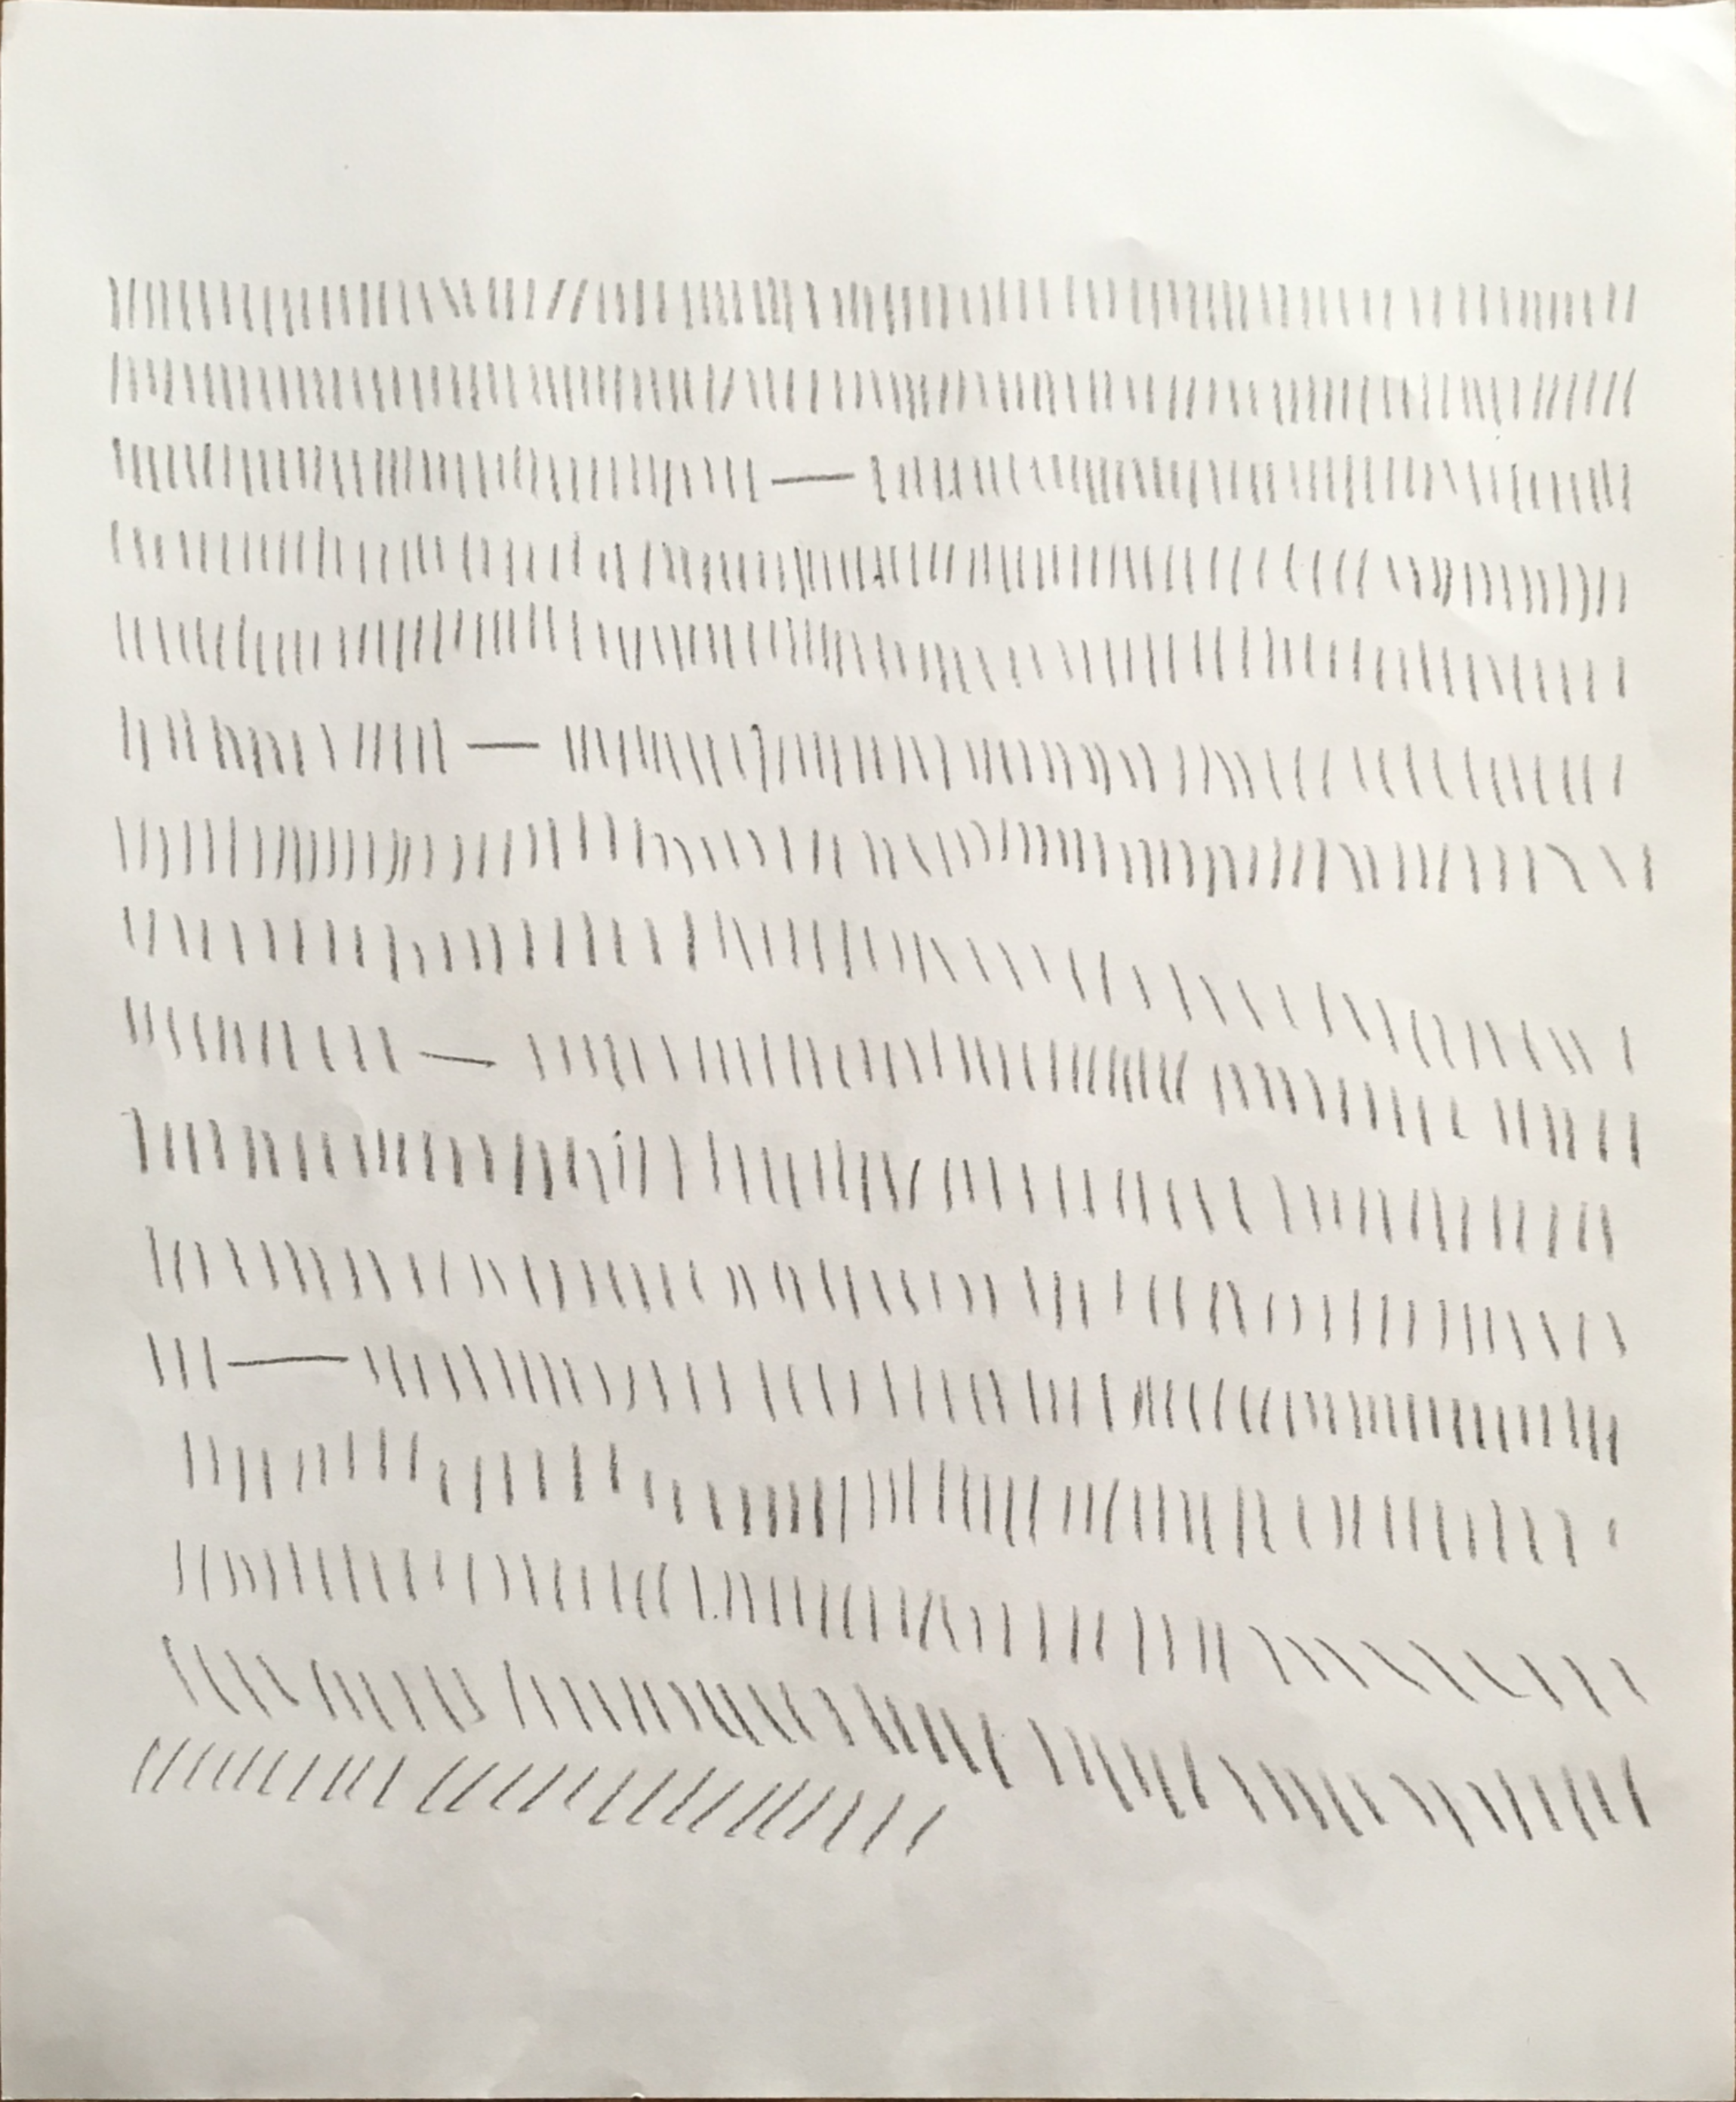
\includegraphics[width=0.40\textwidth]{./fig/desenvolvimento/correcao_perspectiva}
    \label{subfig:img-segmentada}
   }
   \caption{{\subref{subfig:roi-img}} e {\subref{subfig:img-segmentada}} Resultado do processamento segmentação da imagem }
  \label{subfig:segmentacao}
\end{figure}

Após a obtenção das coordenadas da nossa ROI é realizado o processo de segmentação. Nesse processo é realizado a separação entre o objeto detectado e o fundo da imagem, como já temos o vetor com as coordenas (x,y) do objeto, é feito um recorte na imagem original utilizando essas coordenadas realizando assim a segmentação. É realizado também a correção de perspetiva do objeto, utilizando a função \textbf{warpPerspective} da Opencv, isso melhora na detecção dos palos.

\section{Identificação dos palos}
\label{sec:ident-palos}

Após a segmentação da folha com o teste dos palos, são aplicados alguns algoritmos  de melhoria na imagem por histograma e operações morfológicas para que possa se identificar os palos.
\subsection{Pré-processamento}
\label{sec:pre-proce}
Nessa etapa a imagem é convertida para o espaço de cores LAB,  onde a camada L é responsável por armazenar somente os dados de luminosidade da imagem em seguida é aplicado uma correção do contraste por equalização adaptativa do histograma utilizando a função da Opencv \textbf{createCLAHE} essa abordagem é mais eficiente em imagens onde pode haver maior variação de luminosidade, pois o ajuste do contraste por histograma ocorre em pedaços da imagem e não na imagem de maneira global. Em seguida são realizadas  transformações morfológicas  com a função \textbf{morphologyEx} da Opencv foram utilizadas as operações de erosão e dilatação e a \textbf{BLACKHAT}, depois foi aplicado um filtro de suavização  para redução de ruídos, em seguida a imagem foi binarizada utilizando a função \textbf{threshold}.
Na imagem \ref{subfig:roi-seg}  temos o resultado da aplicação dessas técnicas de processamento.

\begin{figure}[h]
 \centering
  \subfigure[][Imagem após equalização adaptativa por histograma.]
   {
    
    \includegraphics[width=0.32\textwidth]{./fig/desenvolvimento//img_clahe}
    \label{subfig:roi-clahe}
   } \qquad
    \subfigure[][Imagem apos aplicação a transformação morfológica BLACKHAT.]
   {
    \includegraphics[width=0.32\textwidth]{./fig/desenvolvimento//blackhat}
    \label{subfig:roi-blck}
   } \qquad
  \subfigure[Imagem binarizada.]
   {
    \includegraphics[width=0.32\textwidth]{./fig/desenvolvimento/binarization}
    \label{subfig:roi-bin}
   }
   \caption{{\subref{subfig:roi-clahe}} , {\subref{subfig:roi-blck}} e {\subref{subfig:roi-bin}} Resultado do processamento e binarização da imagem }
  \label{subfig:roi-seg}
\end{figure}

Após a binarização é utilizado a função \textbf{findContours} da Opencv com os parâmetros \textbf{RETR EXTERNAL}  que diz a função para retornar os contornos mais externos e o parâmetro \textbf{CHAIN APPROX SIMPLE} que utiliza menos pontos para os contornos dos objetos encontrados na imagem, assim como foi feito na parte de localização da folha do teste palográfico, essa função retorna uma lista com as coordenadas x e y de cada objeto encontrado na imagem, no caso, os palos. Porém, ainda pode haver ruído nessa lista, com o objetivo de removê-los, é feito uma validação que remove os objetos que tiverem um valor para o x muito próximo da margem da folha  e cuja área é muito pequena ou muito grande, então são removidos da lista de palos válidos.

\section{Contagem dos palos}
\label{sec:ident-palos}

O processo de contagem dos palos precisa ser linha a linha da direita para esquerda até chegar no traço horizontal, em seguida recomeça-se a contagem e repete-se esse processo para os 5 tempos do teste. Pensando nisso foi desenvolvido um algorítimo que localiza o primeiro palo e a partir dele sempre pega o palo mais próximo. Para isso é calculado a distância entre os palos utilizando as coordenadas cartesianas (x,y) de cada palo. A fórmula utilizada é a distância euclidiana. $d_{ab}=\sqrt{(x_b - x_a)^2 + (y_b - y_a)^2}$  a partir disso é feito a ordenação dos palos para que o processo de contagem fique correto.

Em seguida depois de ordenado os palos é feito a contagem  nos 5 intervalos de tempo. Com essa informação verifica-se a diferença de palos de um intervalo para o outro e somamos essa diferença para calcularmos o NOR (Nível de Oscilação Rítmica e poderíamos calcular a produtividade e fazer o gráfico de rendimento. A imagem \ref{fig:ord-contagem} tem o resultado desse processo.

\begin{figure}[H]
 \centering
 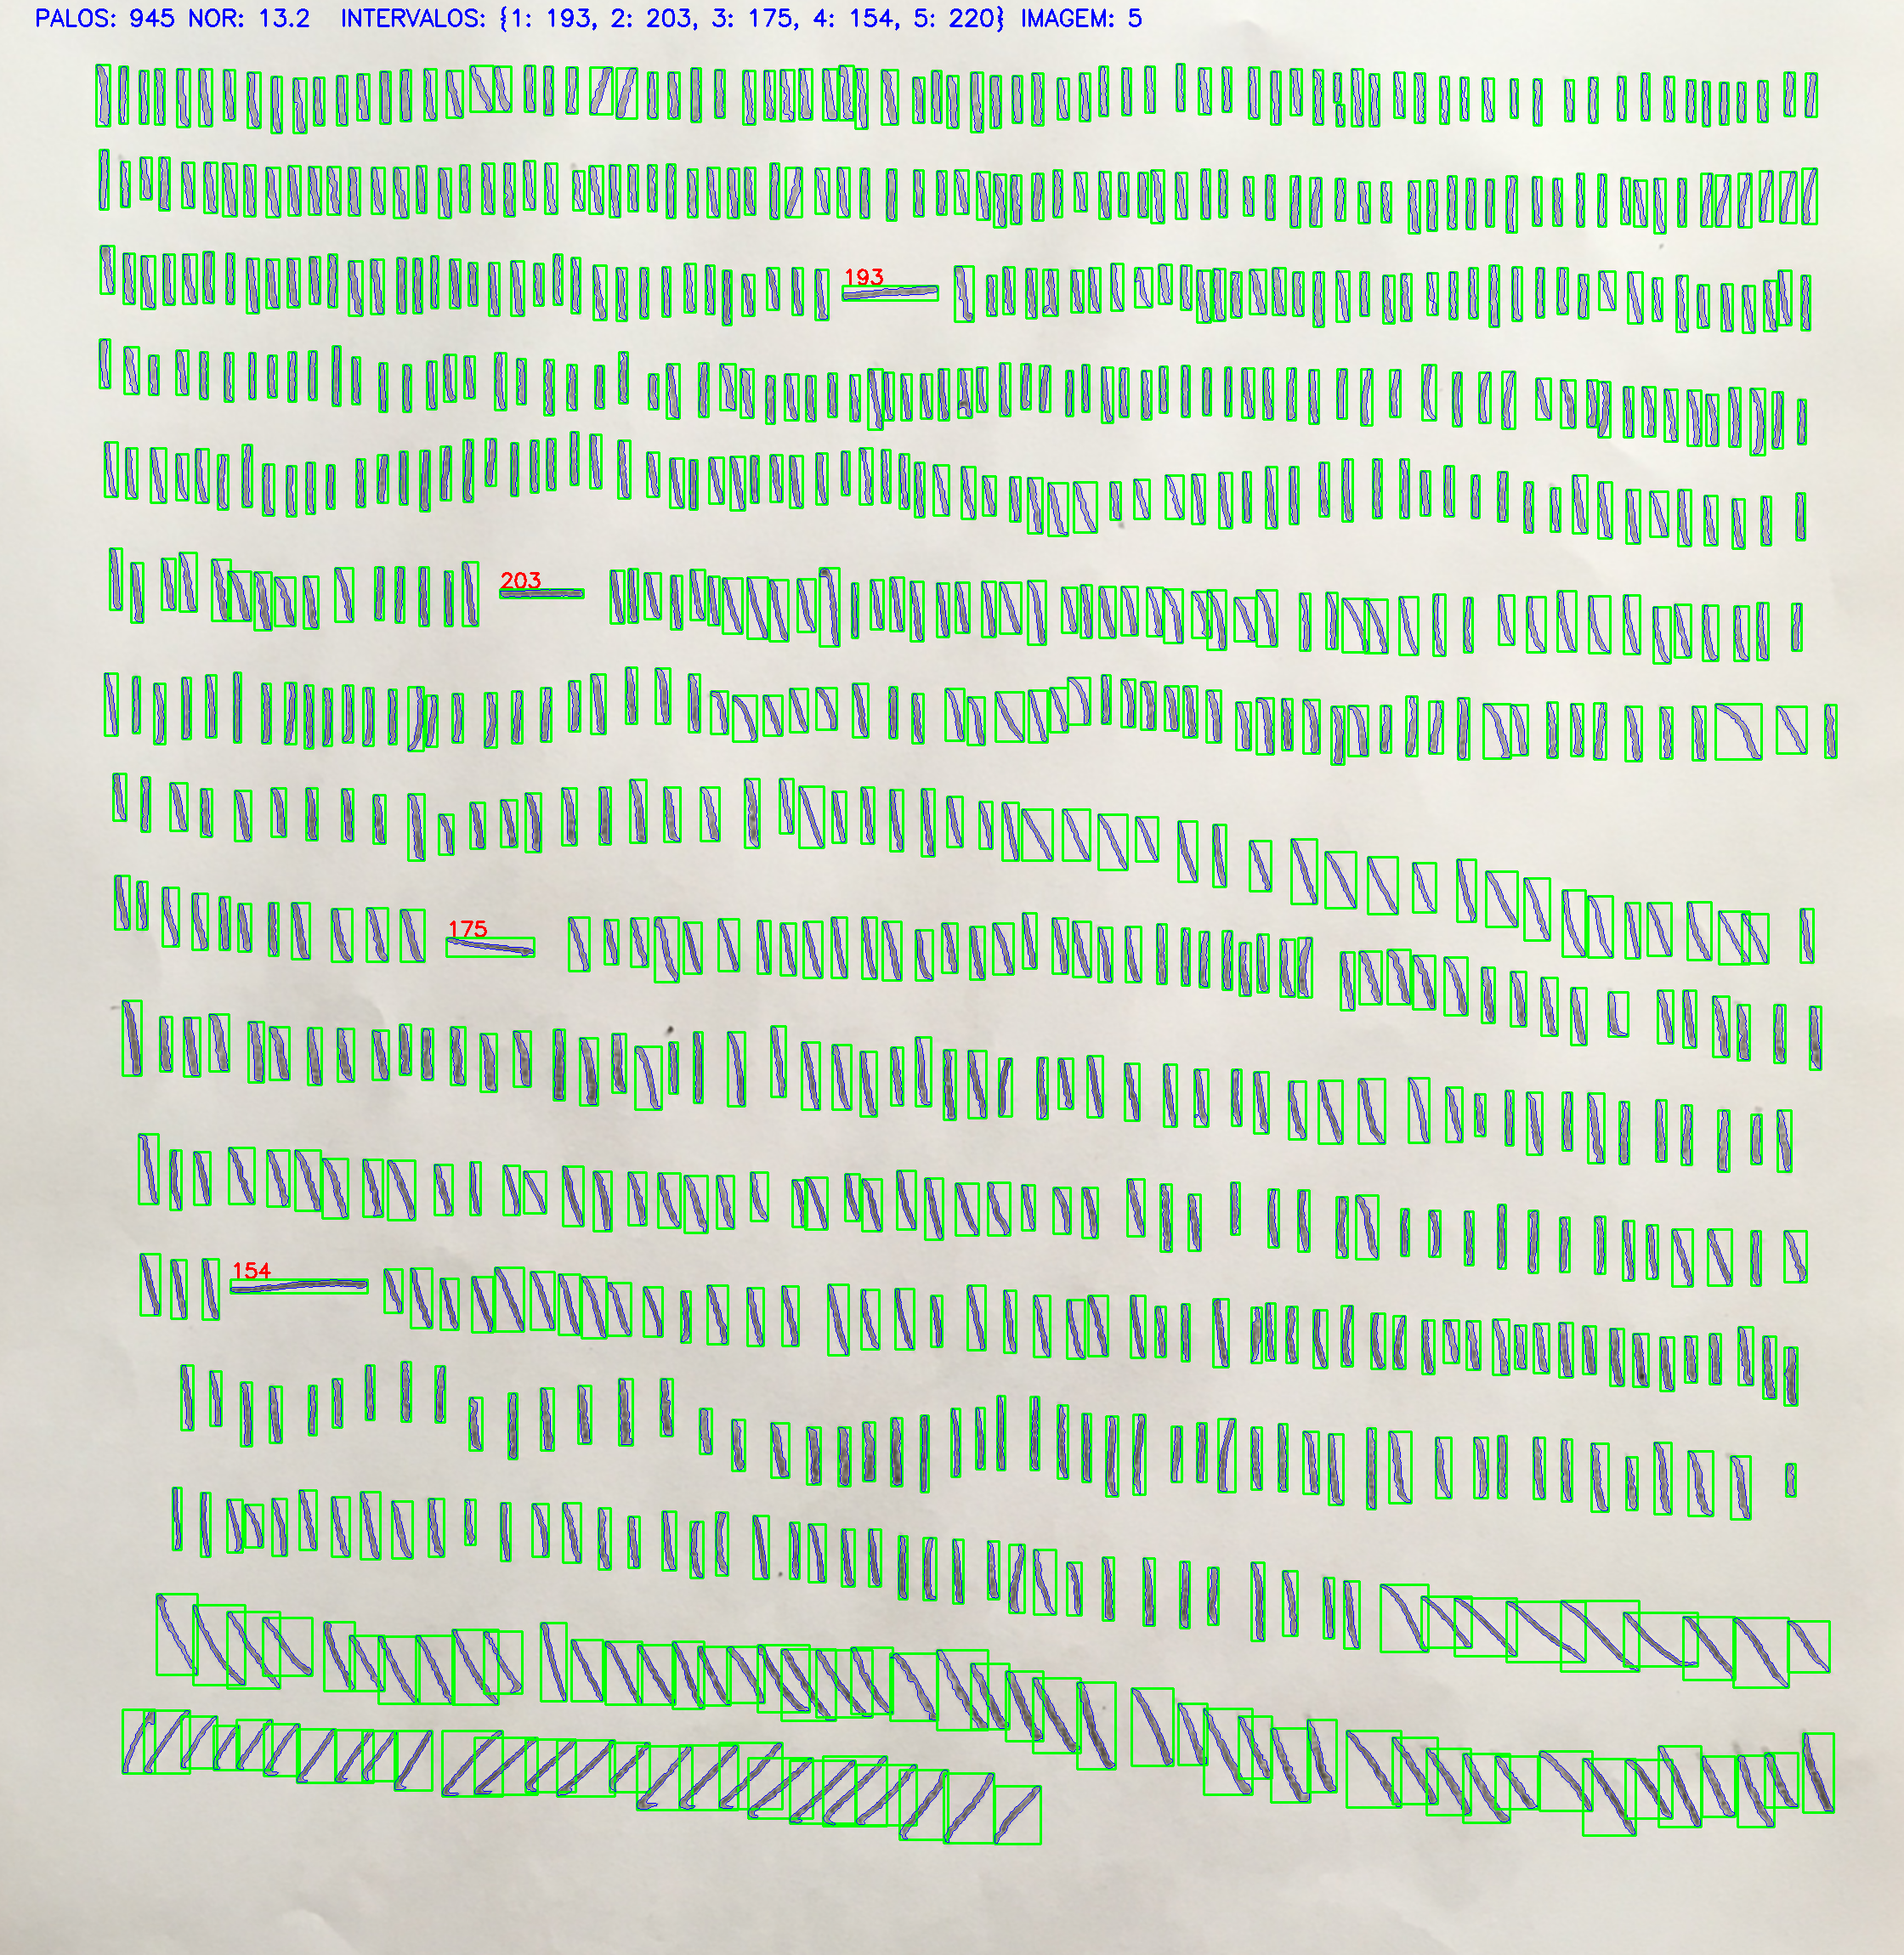
\includegraphics[width=0.70\textwidth]{./fig/desenvolvimento/final}
 \caption{Resultado da ordenação e contagem dos palos.}
 \label{fig:ord-contagem}
\end{figure}





